% Drawing 14/05-1 -- folder 14, batch 05, archive page 95 (PDF page 96).
% Transcription: à droite, un croquis : trois cônes emboîtés de même sommet, figurés par trois ovales emboîtés, tangents entre eux à droite, marqués $P$, $Q$, $R$ de l'extérieur vers l'intérieur, et par des génératrices issues du sommet commun, en bas ; la génératrice de droite, commune aux trois, est épaissie.
% Kind: three nested cones with a common vertex, marked P, Q, R. Method 2 (schematic redraw from the facsimile). Status: ok.
% Notes: As on the page: three nested ovals (the sections of the cones), the larger containing the smaller, all three touching at the right near the heavy generator; the letters P (on the outer one, at the top), Q (on the middle one) and R (inside the inner one); four generators from the common vertex, drawn from that one point: to the left end of the outer oval, to the left end of the middle oval, to the left end of the inner oval, and the heavy one at the right, tangent to the three ovals. Ovals are drawn as ellipses fitted to his outlines. Redrawn 2026-11-12 (issue 128): to check again.
% Coordinates: 1 unit = 0.5 mm = 1/100 of the crop width (bbox in page fractions: [0.78, 0.43, 0.96, 0.57]).
% Redrawn by Claude (claude-fable-5-2), issue #128, 2026-11-12; not checked by a human; not compiled (no TeX in the session).
% Rights: reproduces part of the work -- behind RENDER_TRANSCRIPTS, never published by itself.
\documentclass[tikz,border=3pt]{standalone}
\usepackage{amsmath,amssymb}
\usetikzlibrary{patterns,arrows.meta}
\tikzset{pencil/.style={black!45}, struck/.style={black!35}, mpt/.style={circle,draw,inner sep=1.3pt}, pt/.style={circle,fill,inner sep=0.9pt}, opt/.style={circle,draw,fill=white,inner sep=1.1pt}}
\begin{document}
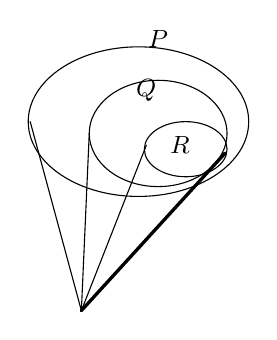
\begin{tikzpicture}[x=0.5mm,y=0.5mm,line cap=round,line join=round,font=\scriptsize]
\draw (48,-40) ellipse[x radius=28, y radius=19];
\draw (53,-43) ellipse[x radius=17.5, y radius=13.5];
\draw (60,-47) ellipse[x radius=10.5, y radius=7];
\draw (33.5,-88) -- (20.5,-40);
\draw (33.5,-88) -- (35.5,-43);
\draw (33.5,-88) -- (50,-46);
\draw[very thick] (33.5,-88) -- (70,-48);
\node[inner sep=1pt] at (53,-19) {\small $P$};
\node[inner sep=1pt] at (50,-32) {\small $Q$};
\node[inner sep=1pt] at (58.5,-46) {\small $R$};
\end{tikzpicture}
\end{document}
